\chapter{函数逼近}
\label{chap:function-approximation}

第~\ref{chap:functions-as-vectors}章把函数看成很长的向量$[\ldots,a_1,a_2,\ldots]$，每个输入占一个分量。计算机却只能存放有限个数，所以实际处理的总是这个长向量的一个低维替身。怎样选替身，替身离原来的函数有多远，就是本章的问题。

有限维的情形我们已经熟悉。在$\mathbb R^3$中，用$xy$平面上的点代替向量$v=(3,4,1)$，最近的点是垂足$(3,4,0)$，误差是
\[
 \lVert(3,4,1)-(3,4,0)\rVert_2=1 .
\]
三个数被压缩成两个，代价正好是被丢掉的那个分量。函数逼近做的是同一件事：候选的“平面”换成多项式、阶梯函数或若干基函数张成的子空间，“垂足”换成候选集合中离目标最近的元素。

这个图景有三个要素：要逼近的目标，量距离的尺子（范数），以及允许使用的低维候选集合。本章沿着三个问题展开。候选集合不断增大时，误差能否趋于零？只给定预算时，最小误差是多少，又怎样随预算下降？同样的预算下，选哪种候选集合最合适？

第~\ref{sec:fapprox-integrable}节回答第一个问题：在$L^p$中，简单函数、连续函数和光滑函数都能以任意精度逼近给定的可积函数，但结论依赖测度、指数$p$，在$L^\infty$中会失效。第~\ref{sec:fapprox-error}节加入预算，用点到集合的距离定义最佳误差，并用Fourier截断说明“丢掉坐标”的代价可以精确算出。

后三节比较三种选择低维替身的方式。第~\ref{sec:fapprox-fixed-subspaces}节在看到目标之前就固定子空间，类似于事先选定一张投影平面。第~\ref{sec:fapprox-best-n-term}节固定坐标轴，却按目标挑选保留哪几个坐标。第~\ref{sec:fapprox-adaptive}节让分点随目标移动，相当于连坐标轴也按目标调整。贯穿的例子是折线$f_*(x)=\lvert x-\frac12\rvert$、平方根$\sqrt x$以及在$3/4$处跳跃的阶梯函数。

有限维的直觉在两处要修正。无限维中任何有限维子空间都离整个空间很远，单位球不紧，所以单个函数的误差趋于零，并不意味着一类函数有共同的速率。不同范数也不再等价，同一个近似用不同的尺子量，结论可以完全不同。

本章只建立误差的定义、构造与基本估计。用导数、尺度或点值刻画目标的正则性，从而给出更精确的误差界，分别由第~\ref{chap:sobolev-spaces}章、第~\ref{chap:besov-spaces}章和第~\ref{chap:rkhs}章承担；从带误差的数据中拟合函数属于卷五。

\section{可积函数的逼近}
\label{sec:fapprox-integrable}

有限维中有一个基本事实：有理分量的向量在$\mathbb R^n$中稠密，任何向量都能被它们以任意精度接近。可积函数这种“无限长的向量”可能处处不连续，也可能无界，我们希望知道它能否被结构简单的函数接近。这样，许多论证就可以先对简单函数验证，再推广到一般函数。

用第~\ref{chap:topological-spaces}章的语言，这是在问某个函数族在$L^p$中是否稠密，能否取到可数的稠密族。第~\ref{chap:metric-spaces}章的距离和点列判据，把问题化为构造一列误差趋于零的近似。本节依次使用简单函数、连续函数和光滑函数，每一步都核对所用的测度、指数$p$与范数。

\subsection{简单函数逼近}
\label{sec:fapprox-simple}

只取有限多个值的可测函数称为简单函数，可以写成
\[
 s=\sum_{i=1}^kc_i\mathbf 1_{A_i},\qquad A_i\ \text{可测},\quad c_i\in\mathbb K .
\]
用向量的话说，这是分量只有有限种不同取值的向量，就像把一个长向量的每个分量四舍五入到有限个档位。第~\ref{chap:measure}章已经用取值分层构造了逐点收敛的简单函数列，这里要问的是：误差用$L^p$范数衡量时，它是否也趋于零。

\paragraph{截断与取值分层}
对非负函数，把取值范围按二进分层，每层取下端点，再把过大的值截断。设$f\geq0$可测，令
\begin{equation}
 s_n=\min\bigl\{n,\ 2^{-n}\lfloor2^nf\rfloor\bigr\},\qquad n=1,2,\ldots .
 \label{eq:fapprox-dyadic-simple}
\end{equation}
这里做了两件事：$\lfloor2^nf\rfloor/2^n$相当于把分量舍入到间距为$2^{-n}$的档位，取$\min$相当于把超过$n$的大分量压到$n$。

在$f$落入$[j2^{-n},(j+1)2^{-n})$的集合上，$s_n$取值$j2^{-n}$；在$f\geq n$的集合上，$s_n$取值$n$。所以$s_n$只取有限多个值。同时，每一点都有
\[
 0\leq s_n\leq f,
\]
并且在$f<n$处有
\[
 0\leq f-s_n<2^{-n}.
\]
$f$有限的点上，$n$足够大后都落在第二种情形，所以$s_n\to f$逐点成立。

\begin{theorem}[简单函数逼近$L^p$函数]
\label{thm:fapprox-simple-dense}
设$(X,\mathcal A,\mu)$为测度空间，$1\leq p<\infty$，$f\in L^p(\mu)$。则存在一列简单函数$s_n=\sum_ic_{n,i}\mathbf 1_{A_{n,i}}$，其中每个$\mu(A_{n,i})<\infty$，使$\lVert f-s_n\rVert_p\to0$。
\end{theorem}

\begin{proof}
先设$f\geq0$，取式~\eqref{eq:fapprox-dyadic-simple}中的$s_n$。$f\in L^p$说明$f$几乎处处有限，于是$\lvert f-s_n\rvert^p\to0$几乎处处成立。又由$0\leq s_n\leq f$，
\[
 \lvert f-s_n\rvert^p\leq f^p ,
\]
右端可积，控制收敛定理给出$\lVert f-s_n\rVert_p\to0$。

再看取值集合的测度。$n\geq1$时，$s_n$的非零取值都不小于$2^{-n}$，所以$\{s_n\neq0\}\subseteq\{f\geq2^{-n}\}$。由Chebyshev不等式，
\[
 \mu(\{s_n\neq0\})\leq\mu(\{f\geq2^{-n}\})\leq2^{np}\lVert f\rVert_p^p<\infty ,
\]
每个非零取值所在的集合测度都有限。

一般的实值$f$写成$f=f^+-f^-$，复值$f$再分实部与虚部。每一部分分别按上面逼近，组合后的误差由三角不等式控制，取值集合仍测度有限。
\end{proof}

这里$p<\infty$用了两次：控制收敛需要$f^p$可积，有限测度的支撑来自Chebyshev不等式。结论只说明简单函数在$L^p(\mu)$中稠密，并没有给出可数的稠密族，因为可测集$A_{n,i}$可以有不可数多种选法。

\begin{example}[两部分误差的大小]
取$(0,1]$上的$f(x)=x^{-1/3}$，$p=2$。它无界，但$\int_0^1x^{-2/3}\,\mathrm dx=3$，所以$f\in L^2$。我们把误差分成被截断的部分和分层舍入的部分分别计算。

$f\geq n$等价于$x\leq n^{-3}$。在这一段上$s_n=n$，平方误差是
\[
 \int_0^{n^{-3}}\bigl(x^{-1/3}-n\bigr)^2\,\mathrm dx
 =\Bigl[3x^{1/3}-3nx^{2/3}+n^2x\Bigr]_0^{n^{-3}}.
\]
代入上限，三项依次是$3/n$、$-3/n$、$1/n$，所以
\[
 \int_0^{n^{-3}}\bigl(x^{-1/3}-n\bigr)^2\,\mathrm dx=\frac1n .
\]

在其余部分，逐点误差小于$2^{-n}$，区间长度不超过$1$，平方误差不超过$4^{-n}$。合起来，
\[
 \lVert f-s_n\rVert_2^2\leq\frac1n+4^{-n}.
\]
$n=2$时右端是$0.5+0.0625$，$n=10$时约为$0.1$。舍入误差按指数下降，真正慢的是截断带来的误差。

若把$p=2$换成$p=3$，则$\int_0^1x^{-1}\,\mathrm dx=\infty$，$f$不属于$L^3$，定理不适用。此时被截断部分的三次积分也发散，误差始终是无穷大。
\end{example}

\paragraph{Lebesgue区域上的可数逼近族}
$\mathbb R^n$中用有理分量得到可数稠密集。在欧氏空间的函数上，同样的想法分两步：可测集用矩形逼近，矩形和系数都只取有理数。设$\Omega\subseteq\mathbb R^d$可测，取Lebesgue测度$\lambda$。称各边端点都是有理数的矩形$R=\prod_{i=1}^d[a_i,b_i)$为有理矩形，令$\mathcal D$为全体有限和
\[
 \sum_{i=1}^kc_i\mathbf 1_{R_i\cap\Omega},\qquad R_i\ \text{为有理矩形},\quad \operatorname{Re}c_i,\operatorname{Im}c_i\in\mathbb Q .
\]
有理矩形只有可数多个，系数也只有可数多种，所以$\mathcal D$可数。

\begin{theorem}[$L^p(\Omega)$的可数稠密族]
\label{thm:fapprox-separable}
在上述记号下，设$1\leq p<\infty$，则$\mathcal D$在$L^p(\Omega)$中稠密，因而$L^p(\Omega)$可分。
\end{theorem}

\begin{proof}
先化简目标。由定理~\ref{thm:fapprox-simple-dense}和三角不等式，只需逼近有限测度可测集$A\subseteq\Omega$的示性函数，系数换成有理复数只带来任意小的误差。对有理矩形的有限并$U$，有
\[
 \lVert\mathbf 1_A-\mathbf 1_{U\cap\Omega}\rVert_p^p=\lambda\bigl(A\mathbin{\triangle}(U\cap\Omega)\bigr)\leq\lambda(A\mathbin{\triangle}U),
\]
所以只需对任意$\varepsilon>0$，找到$U$使$\lambda(A\mathbin{\triangle}U)$小于$3\varepsilon$。

第一步，用可数个矩形覆盖$A$。由Lebesgue测度的定义（第~\ref{chap:measure}章），存在矩形$R_1,R_2,\ldots$覆盖$A$，并且$\sum_i\lambda(R_i)<\lambda(A)+\varepsilon$。于是
\[
 \lambda\Bigl(\bigcup_iR_i\setminus A\Bigr)<\varepsilon .
\]

第二步，截成有限个。级数收敛，取$N$使$\sum_{i>N}\lambda(R_i)<\varepsilon$，令$U_0=\bigcup_{i\leq N}R_i$。由$A\setminus U_0\subseteq\bigcup_{i>N}R_i$，$\lambda(A\setminus U_0)<\varepsilon$。又$U_0\setminus A\subseteq\bigcup_iR_i\setminus A$，合起来
\[
 \lambda(A\mathbin{\triangle}U_0)<2\varepsilon .
\]

第三步，把端点换成有理数。把每个$R_i$（$i\leq N$）放大成有理矩形$R_i'\supseteq R_i$，使$\lambda(R_i'\setminus R_i)<\varepsilon/N$，这只需把各端点向外移到足够近的有理数。令$U=\bigcup_{i\leq N}R_i'$，则$\lambda(U\setminus U_0)<\varepsilon$，所以
\[
 \lambda(A\mathbin{\triangle}U)<3\varepsilon .
\]
最后，有限个有理矩形的并可以用所有端点坐标切成有限个两两不交的有理矩形，因此$\mathbf 1_{U\cap\Omega}$属于$\mathcal D$。
\end{proof}

\paragraph{一般测度空间的条件}
上面的证明只用到一点：存在可数个有限测度集组成的族，使每个有限测度可测集都能用其中有限个的并按测度逼近。一般测度空间中这需要另外核对。

反例是不可数集$I$上的计数测度，此时$L^p$就是$\ell^p(I)$。这个“向量”有不可数个分量，单点示性函数$\mathbf 1_{\{i\}}$是坐标向量，两两距离为$2^{1/p}$。以它们为中心、半径$2^{1/p}/2$的开球两两不交且有不可数个，而稠密子集必须在每个球中都有元素，所以不存在可数稠密子集。

\paragraph{有界函数与本质上确界}
$p=\infty$时情况又不同。$L^\infty$范数相当于取向量各分量绝对值的最大值，这把尺子不允许任何一段上的误差被平均掉。在$L^\infty[0,1]$中取$f_t=\mathbf 1_{[0,t]}$，$0<t<1$。对$s<t$，差$f_t-f_s=\mathbf 1_{(s,t]}$在正测度集上等于$1$，所以
\[
 \lVert f_t-f_s\rVert_\infty=1 .
\]
半径$1/2$的球$\{g:\lVert g-f_t\rVert_\infty<1/2\}$两两不交，共有不可数个，同样的论证说明$L^\infty[0,1]$没有可数稠密子集。

但简单函数在$L^\infty$中仍然稠密。设$f$是实值本质有界函数，取一个满足$\lvert f\rvert\leq M$处处成立的代表。取$n\geq M$，对$f^+$与$f^-$分别作式~\eqref{eq:fapprox-dyadic-simple}的分层，组合后得到$s_n$，于是
\[
 \lVert f-s_n\rVert_\infty\leq2^{-n}.
\]
复值时分实部与虚部处理。

这两个结论并不矛盾。这里的简单函数，其取值集合是$f$的水平集，可以有不可数多种，无法取成可数族；可数的有理矩形虽然能按测度逼近这些集合，却控制不了本质上确界：把集合修改一小块，$L^\infty$误差仍可能是$1$。

\subsection{光滑函数逼近}
\label{sec:fapprox-smooth}

简单函数一般不连续。许多论证希望先对连续甚至光滑的函数推导，例如把导数移到另一个函数上，再推广到一般函数。本小节在欧氏开集$\Omega\subseteq\mathbb R^d$上取Lebesgue测度，分三步建立这种逼近：先用集合的开紧逼近得到连续函数，再证明平移在$L^p$中连续，最后用第~\ref{chap:smoothing-weak-derivatives}章的卷积磨光得到光滑函数。

\paragraph{紧支撑连续函数}
记$C_c(\Omega)$为$\Omega$上支撑为紧集的连续函数。第~\ref{chap:smoothing-weak-derivatives}章由矩形覆盖推出了Lebesgue测度的正则性：对有限测度可测集$A\subseteq\Omega$和$\varepsilon>0$，存在紧集$K$与开集$U$，使$K\subseteq A\subseteq U\subseteq\Omega$且$\lambda(U\setminus K)<\varepsilon$。于是示性函数$\mathbf 1_A$的棱角可以夹在$K$与$U$之间用一个连续的“斜坡”磨掉。

\begin{theorem}[紧支撑连续函数逼近$L^p$函数]
\label{thm:fapprox-cc-dense}
设$\Omega\subseteq\mathbb R^d$为开集，$1\leq p<\infty$，则$C_c(\Omega)$在$L^p(\Omega)$中稠密。
\end{theorem}

\begin{proof}
由定理~\ref{thm:fapprox-simple-dense}，只需逼近有限测度集$A\subseteq\Omega$的示性函数。按上面的正则性取$K\subseteq A\subseteq U$，$\lambda(U\setminus K)<\varepsilon$。若$K$是空集，取$\varphi=0$，此时误差的$p$次方不超过$\lambda(U)<\varepsilon$。下设$K$非空。

为使连续函数有紧支撑，先把$U$缩小。$K$紧且含于开集$\Omega$，它到$\Omega$的补集有正距离（$\Omega=\mathbb R^d$时这一距离取为$+\infty$）。取$\delta>0$小于这个距离，令
\[
 U'=U\cap\{x:\operatorname{dist}(x,K)<\delta\}.
\]
$U'$仍是包含$K$的开集，它的闭包含于有界闭集
\[
 \{x:\operatorname{dist}(x,K)\leq\delta\}\subseteq\Omega ,
\]
因而是$\Omega$内的紧集。

定义斜坡函数
\[
 \varphi(x)=\frac{\operatorname{dist}(x,U'^c)}{\operatorname{dist}(x,U'^c)+\operatorname{dist}(x,K)} .
\]
$K$与闭集$U'^c$不交，分母处处为正，所以$\varphi$连续。它在$K$上等于$1$，在$U'$外等于$0$，取值在$[0,1]$中，支撑含于$U'$的闭包，因而$\varphi\in C_c(\Omega)$。

最后估计误差。$\mathbf 1_A$与$\varphi$在$K$上都等于$1$，在$U$外都等于$0$，所以$\mathbf 1_A-\varphi$只在$U\setminus K$上可能非零，并且绝对值不超过$1$。于是
\[
 \lVert\mathbf 1_A-\varphi\rVert_p^p\leq\lambda(U\setminus K)<\varepsilon .
\]
\end{proof}

\paragraph{平移的$L^p$连续性}
磨光是对附近的平移作平均，所以要先知道小平移在$L^p$范数下改变函数多少。对长向量来说，平移就是把所有分量的下标错开一位。记$(\tau_hf)(x)=f(x-h)$。Lebesgue测度在平移下不变，所以$\lVert\tau_hf\rVert_p=\lVert f\rVert_p$。第~\ref{chap:smoothing-weak-derivatives}章对$p=1$证明了平移的积分连续性，下面对一般有限$p$给出同样的结论。

\begin{theorem}[平移在$L^p$中连续]
\label{thm:fapprox-translation}
设$1\leq p<\infty$，$f\in L^p(\mathbb R^d)$，则$\lVert\tau_hf-f\rVert_p\to0$（$h\to0$）。
\end{theorem}

\begin{proof}
先设$g\in C_c(\mathbb R^d)$，支撑含于球$B_R$。$g$一致连续，记
\[
 \omega_g(t)=\sup_{\lvert x-y\rvert\leq t}\lvert g(x)-g(y)\rvert ,
\]
则$\omega_g(t)\to0$。对$\lvert h\rvert\leq1$，$\tau_hg-g$的支撑含于$B_{R+1}$，所以
\[
 \lVert\tau_hg-g\rVert_p^p\leq\omega_g(\lvert h\rvert)^p\,\lambda(B_{R+1})\to0 .
\]

一般地，任给$\varepsilon>0$，由定理~\ref{thm:fapprox-cc-dense}取$g\in C_c(\mathbb R^d)$使$\lVert f-g\rVert_p<\varepsilon$。三角不等式把$\tau_hf-f$分成三段：
\[
 \lVert\tau_hf-f\rVert_p\leq\lVert\tau_h(f-g)\rVert_p+\lVert\tau_hg-g\rVert_p+\lVert g-f\rVert_p .
\]
由平移不变性，第一项等于$\lVert f-g\rVert_p<\varepsilon$；第三项也小于$\varepsilon$。于是
\[
 \lVert\tau_hf-f\rVert_p<2\varepsilon+\lVert\tau_hg-g\rVert_p ,
\]
最后一项在$h$充分小时小于$\varepsilon$。
\end{proof}

$p=\infty$时结论不成立。在$\mathbb R$上取$f=\mathbf 1_{[0,1/2]}$。对$0<\lvert h\rvert<1/2$，$\tau_hf-f$在两个长为$\lvert h\rvert$的区间上取值$\pm1$，所以
\[
 \lVert\tau_hf-f\rVert_\infty=1 .
\]
积分范数允许误差集中在测度很小的集合上，本质上确界不允许。

\paragraph{磨光的$L^p$收敛}
取第~\ref{chap:smoothing-weak-derivatives}章的磨光核：$\rho$光滑、非负、积分为$1$、支撑于单位闭球，缩放后记为
\[
 \rho_\varepsilon(x)=\varepsilon^{-d}\rho(x/\varepsilon).
\]
那里证明了$f_\varepsilon=\rho_\varepsilon*f$光滑，并在$L^1$意义下局部逼近$f$。用向量的话说，$f_\varepsilon$是对相邻分量做加权滑动平均；下面在全空间上证明$L^p$收敛，误差由平移误差控制。

\begin{theorem}[磨光在$L^p$中收敛]
\label{thm:fapprox-mollifier}
设$1\leq p<\infty$，$f\in L^p(\mathbb R^d)$，$f_\varepsilon=\rho_\varepsilon*f$。则
\begin{equation}
 \lVert f_\varepsilon-f\rVert_p\leq\sup_{\lvert h\rvert\leq\varepsilon}\lVert\tau_hf-f\rVert_p\to0\qquad(\varepsilon\to0).
 \label{eq:fapprox-mollifier-error}
\end{equation}
\end{theorem}

\begin{proof}
由$\int\rho_\varepsilon=1$，可以把$f(x)$写进平均里：
\[
 f_\varepsilon(x)-f(x)=\int\rho_\varepsilon(h)\bigl(f(x-h)-f(x)\bigr)\,\mathrm dh .
\]

$p>1$时记$q=p/(p-1)$，把被积函数写成$\rho_\varepsilon^{1/q}\cdot\rho_\varepsilon^{1/p}\lvert f(x-h)-f(x)\rvert$。由Hölder不等式与$\int\rho_\varepsilon=1$，
\[
 \lvert f_\varepsilon(x)-f(x)\rvert^p\leq\int\rho_\varepsilon(h)\,\lvert f(x-h)-f(x)\rvert^p\,\mathrm dh .
\]
$p=1$时这就是绝对值不等式。

被积函数非负可测，对$x$积分并由Tonelli定理交换积分次序，
\[
 \lVert f_\varepsilon-f\rVert_p^p\leq\int\rho_\varepsilon(h)\,\lVert\tau_hf-f\rVert_p^p\,\mathrm dh .
\]
$\rho_\varepsilon$支撑于半径$\varepsilon$的闭球且积分为$1$，所以右端是$\lVert\tau_hf-f\rVert_p^p$的加权平均，不超过它在$\lvert h\rvert\leq\varepsilon$上的上确界。由定理~\ref{thm:fapprox-translation}，这一上确界随$\varepsilon\to0$趋于零。
\end{proof}

跳跃函数最能说明指数$p$的作用。取$\mathbb R$上的$f=\mathbf 1_{[0,1/2]}$，当$\varepsilon\leq1/4$时，$f_\varepsilon-f$只集中在两个跳跃点两侧宽$\varepsilon$的带内。记$T(u)=\int_u^1\rho(v)\,\mathrm dv$，代换$x=\varepsilon u$后，两个跳跃点各贡献两段相同的积分，得到
\[
 \lVert f_\varepsilon-f\rVert_p^p=4\varepsilon\int_0^1T(u)^p\,\mathrm du .
\]

所以$L^p$误差按$\varepsilon^{1/p}$下降：$p=1$时是一阶，$p=2$时是$\varepsilon^{1/2}$。$p$越大，指数$1/p$越小。到$p=\infty$，指数变成零，而跳跃点处$f_\varepsilon$的值恒为$1/2$，误差$1/2$不再变化。图~\ref{fig:fapprox-mollifier-norms}把这件事画了出来：曲线明显向跳跃靠拢，$L^1$与$L^2$的误差都在下降，一致误差却保持不动。

\begin{BookInlineFigure}
  \centering
  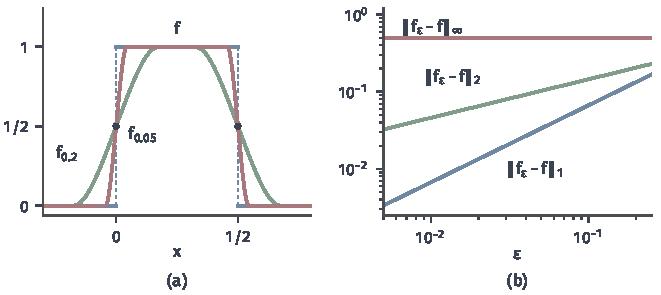
\includegraphics[width=112mm]{figures/04-spaces-measures-and-geometry/03-function-spaces/matplotlib/fapprox-mollifier-norms/figure.pdf}
  \caption{跳跃函数的磨光。(a)$f=\mathbf 1_{[0,1/2]}$（蓝）与$\varepsilon=0.2$（绿）、$\varepsilon=0.05$（红）的磨光；两个黑点标出无论$\varepsilon$多小，$f_\varepsilon$在跳跃点都等于$1/2$。(b)三种范数下的误差随$\varepsilon$的变化，双对数坐标：$L^1$误差为$2m_1\varepsilon$（$m_1\approx0.3345$），$L^2$误差正比于$\varepsilon^{1/2}$，$L^\infty$误差恒为$1/2$。}
  \label{fig:fapprox-mollifier-norms}
\end{BookInlineFigure}

\paragraph{光滑紧支撑函数与局部逼近}
两步合起来就得到光滑函数的逼近。设$f\in L^p(\Omega)$，$1\leq p<\infty$，$\varepsilon_0>0$。由定理~\ref{thm:fapprox-cc-dense}取$g\in C_c(\Omega)$使$\lVert f-g\rVert_p<\varepsilon_0$，把$g$在$\Omega$外延拓为零。

$\rho_\varepsilon*g$光滑，支撑含于$\operatorname{supp}g$的$\varepsilon$邻域。取$\varepsilon$小于$\operatorname{supp}g$到$\Omega^c$的距离，它就属于$C_c^\infty(\Omega)$。由定理~\ref{thm:fapprox-mollifier}，再取$\varepsilon$足够小，使$\lVert\rho_\varepsilon*g-g\rVert_p<\varepsilon_0$。所以$C_c^\infty(\Omega)$在$L^p(\Omega)$（$1\leq p<\infty$）中稠密。

只在局部可积的函数也有局部版本，办法是先截断。设$f\in L^p_{\mathrm{loc}}(\Omega)$，即在每个紧集上$p$次可积，$K\subset\Omega$紧。取$\delta>0$使闭邻域
\[
 K_\delta=\{x:\operatorname{dist}(x,K)\leq\delta\}
\]
含于$\Omega$，令$F=f\mathbf 1_{K_\delta}$，则$F\in L^p(\mathbb R^d)$。

对$\varepsilon<\delta$和$x\in K$，$\rho_\varepsilon(x-\cdot)$的支撑落在$K_\delta$内，所以$(\rho_\varepsilon*F)(x)=f_\varepsilon(x)$。由定理~\ref{thm:fapprox-mollifier}，
\[
 \int_K\lvert f_\varepsilon-f\rvert^p\,\mathrm dx\leq\lVert\rho_\varepsilon*F-F\rVert_p^p\to0 .
\]
截断把局部问题化为全空间问题，代价是结论只在远离边界的紧集上成立。

\paragraph{$L^\infty$中的失效}
连续函数在$L^\infty$中不稠密，光滑函数更是如此。在$(0,1)$上取$f=\mathbf 1_{(0,1/2]}$。设$g$连续且$\lVert g-f\rVert_\infty=r$，则下面两个不等式都几乎处处成立：
\[
 g\geq1-r\ \text{在}\ (0,1/2)\ \text{上},\qquad g\leq r\ \text{在}\ (1/2,1)\ \text{上}.
\]
满测度集在区间中稠密，由连续性这两个不等式在相应闭区间上处处成立。取$x=1/2$，得到
\[
 1-r\leq g(1/2)\leq r ,
\]
即$r\geq1/2$。所以任何连续函数与$f$的本质上确界距离都不小于$1/2$，这正是跳跃幅度的一半。

本节的结论都是定性的：对每个精度都存在某个近似，但没有说明近似需要多少参数。简单函数要多少层、磨光宽度要多小，取决于目标函数本身，而定理没有给出任何速率。要比较不同表示的效率，必须先固定允许使用多少参数，这是下一节的任务。

\section{逼近误差}
\label{sec:fapprox-error}

上一节说“存在误差小于$\varepsilon$的近似”，却允许近似的复杂程度随$\varepsilon$任意增长。回到章首的投影图景：要谈“替身离目标多远”，先要定下目标、尺子和允许的候选集合。本节先用候选集合定义最佳可能误差，把它同具体构造得到的误差分开；再比较候选集合是否为线性子空间、尺子是否由内积给出；最后用Fourier截断，把“丢掉坐标”的代价逐项算出来。

\subsection{目标、误差与表示预算}
\label{sec:fapprox-budget}

设$X$是赋范函数空间，$f\in X$是目标。对每个预算$N$，规定一个候选集合$\mathcal A_N\subseteq X$，它包含所有“用预算$N$能写出的函数”。预算可以是线性子空间的维数，可以是展开中允许保留的项数，也可以是分段函数的段数。

要比较候选集合的好坏，最公平的度量是其中最好的那个候选能做到多好。下面的定义就是把点到集合的距离搬到函数上。

\begin{definition}[最佳逼近误差]
\label{def:fapprox-best-error}
对$f\in X$与候选集合$\mathcal A_N\subseteq X$，称
\begin{equation}
 E(f,\mathcal A_N)_X=\inf_{g\in\mathcal A_N}\lVert f-g\rVert_X
 \label{eq:fapprox-best-error}
\end{equation}
为$f$在$\mathcal A_N$中的\term{最佳逼近误差}（error of best approximation）。
\end{definition}

这就是第~\ref{chap:metric-spaces}章的点到集合的距离。由那里的序列判据，$E(f,\mathcal A_N)_X=0$当且仅当$f$属于$\mathcal A_N$的闭包。若$\mathcal A_N$随$N$递增且并集稠密，上一节的结论就可以重述为$E(f,\mathcal A_N)_X\to0$。

最佳误差是在所有候选中取下确界，不依赖任何具体的选法。某个具体构造（例如在结点处插值）得到的误差只是它的一个上界。后面要反复区分这两者。

\paragraph{三种预算}
三种常见预算给出性质不同的候选集合。次数小于$N$的多项式组成$N$维线性空间，好比$\mathbb R^n$中一张固定的$N$维平面。

给定一组标准正交基后，至多用其中$N$个基向量的线性组合组成的集合就不同了。$\mathbb R^2$中$N=1$时，它是两条坐标轴的并，不是平面也不是直线；$e_1$与$e_2$都只用一项，和$e_1+e_2$却要两项。区间上至多$N$段的分段常数函数，若分点可以任意移动，同样不对加法封闭。

后两种集合对数乘封闭，但对加法不封闭，相应的逼近称为\term{非线性逼近}（nonlinear approximation），以区别于在固定线性空间中进行的线性逼近。

\paragraph{单个函数与函数类}
有时我们要的不是某一个函数的误差，而是对一整类函数$\mathcal F$同时有效的保证。此时考虑最坏情形
\begin{equation}
 E(\mathcal F,\mathcal A_N)_X=\sup_{f\in\mathcal F}E(f,\mathcal A_N)_X .
 \label{eq:fapprox-worst-case}
\end{equation}

两者可以相差很多，这也是无限维与有限维差别最明显的地方。设$H$是可分无限维Hilbert空间，$(e_n)$为标准正交基，$V_N=\operatorname{span}\{e_1,\ldots,e_N\}$。对每个$f$，有
\[
 E(f,V_N)^2=\sum_{n>N}\lvert\langle e_n,f\rangle\rvert^2\to0 .
\]
可是对闭单位球$\mathcal F$，取$f=e_{N+1}$，它与$V_N$垂直，距离为$1$，所以
\[
 E(\mathcal F,V_N)=1\qquad\text{对每个}\ N.
\]
单个函数的误差都趋于零，整个单位球却没有共同的速率。在$\mathbb R^n$中，取$V_n$就把全空间装下了，这种现象不会发生。

要得到统一速率，函数类本身必须足够“小”。这与第~\ref{chap:function-class-covers}章的有限覆盖直接相关：若候选集合$\mathcal A$是至多$N$个函数组成的有限集，最坏误差不超过$\varepsilon$恰好说明以$\mathcal A$中各点为中心、半径为$\varepsilon$的闭球覆盖$\mathcal F$。

反过来，若$\mathcal F$能被$N$个半径为$\varepsilon$的闭球覆盖，以这些球心为$\mathcal A$，最坏误差就不超过$\varepsilon$。覆盖数因此恰好描述了用$N$个固定函数逼近整个函数类所能达到的最坏误差。

\subsection{固定空间中的最佳逼近}
\label{sec:fapprox-fixed-space}

最常见的预算是维数。取一列嵌套的有限维子空间$V_1\subseteq V_2\subseteq\cdots\subseteq X$，$\dim V_N\leq N$，研究$E(f,V_N)_X$。一个基本的问题是：下确界能否取到，也就是最近点是否存在。

\begin{theorem}[有限维子空间中最佳逼近的存在]
\label{thm:fapprox-existence}
设$X$为赋范空间，$V\subseteq X$为有限维子空间，$f\in X$。则存在$g^*\in V$使$\lVert f-g^*\rVert=E(f,V)_X$。
\end{theorem}

\begin{proof}
记$d=E(f,V)_X$，取$g_n\in V$使$\lVert f-g_n\rVert\to d$。$n$充分大时，$\lVert f-g_n\rVert\leq d+1$，于是
\[
 \lVert g_n\rVert\leq\lVert f\rVert+\lVert f-g_n\rVert\leq\lVert f\rVert+d+1 .
\]
$(g_n)$是有限维空间中的有界序列。有限维赋范空间中有界闭集是紧集，所以有子列收敛到某个$g^*\in V$。范数连续，取极限得
\[
 \lVert f-g^*\rVert=\lim_k\lVert f-g_{n_k}\rVert=d .
\]
\end{proof}

证明的关键是有限维的闭球紧。这个定理对$V$的维数有实质要求：无限维子空间中最近点可能不存在，第~\ref{chap:function-inner-product-spaces}章用完备性和平行四边形恒等式才在Hilbert空间中重新得到它。

存在不等于唯一，尺子的形状决定了最近点的个数。在$\mathbb R^2$上取最大值范数（两个分量绝对值的较大者），$V=\operatorname{span}\{(0,1)\}$，$f=(1,0)$。对候选$(0,t)$，
\[
 \lVert f-(0,t)\rVert_\infty=\max\{1,\lvert t\rvert\},
\]
对所有$\lvert t\rvert\leq1$都取到最小值$1$，最佳逼近有无穷多个。

图~\ref{fig:fapprox-nearest-point}说明了原因。以$f$为中心把球吹大，第一次碰到$V$的地方就是最近点。欧氏球是圆，碰到直线只有一点；最大值范数的球是正方形，它的一条边整个贴上了直线。

\begin{BookInlineFigure}
  \centering
  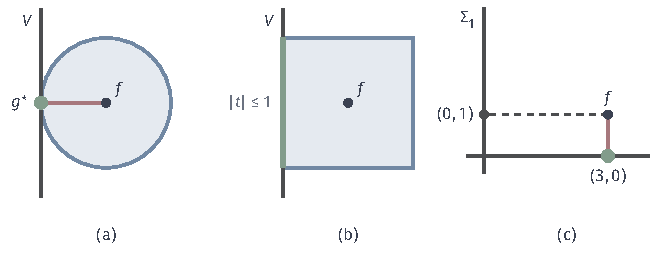
\includegraphics[width=110.882mm]{figures/04-spaces-measures-and-geometry/03-function-spaces/tikz/fapprox-nearest-point/figure.pdf}
  \caption{候选集合与尺子决定最近点。(a)$\mathbb R^2$中欧氏范数：以$f=(1,0)$为中心的圆第一次碰到直线$V$时只有一个切点$g^*$（绿）。(b)最大值范数：同样的半径下，球是正方形，整条边$\{(0,t):\lvert t\rvert\leq1\}$（绿）都是最近点。(c)候选集合$\Sigma_1$是两条坐标轴的并，并非子空间；对$f=(3,1)$，到横轴的距离$1$（红）小于到纵轴的距离$3$（虚线），最近点是$(3,0)$。}
  \label{fig:fapprox-nearest-point}
\end{BookInlineFigure}

\paragraph{Hilbert空间中的正交投影}
内积给出的尺子最好用。由第~\ref{chap:function-inner-product-spaces}章，对闭子空间$V$，正交投影$P_V$给出唯一的最佳逼近，误差满足勾股关系
\begin{equation}
 E(f,V)^2=\lVert f-P_Vf\rVert^2=\lVert f\rVert^2-\lVert P_Vf\rVert^2 .
 \label{eq:fapprox-pythagoras}
\end{equation}
若$V$有标准正交基$e_1,\ldots,e_N$，则投影公式就是把分量读出来：
\[
 P_Vf=\sum_{n\leq N}\langle e_n,f\rangle e_n .
\]
映射$f\mapsto P_Vf$是线性的，这正是后面截断误差可以逐项计算的原因。

\begin{example}[把$x^2$投影到一次函数]
在$L^2[0,1]$中，用次数不超过$1$的多项式逼近$f(x)=x^2$。这个二维子空间有标准正交基
\[
 e_1(x)=1,\qquad e_2(x)=\sqrt{12}\Bigl(x-\frac12\Bigr).
\]

读出$f$在两个方向上的分量：
\[
 \langle e_1,f\rangle=\frac13,\qquad
 \langle e_2,f\rangle=\sqrt{12}\Bigl(\frac14-\frac16\Bigr)=\frac1{\sqrt{12}}.
\]
代入投影公式，$\sqrt{12}$约去，
\[
 P_Vf(x)=\frac13+x-\frac12=x-\frac16 .
\]

误差由式~\eqref{eq:fapprox-pythagoras}得到，只需做减法，这和$\mathbb R^3$中用勾股定理求点到平面的距离一样：
\[
 E(f,V)^2=\frac15-\frac19-\frac1{12}=\frac1{180}.
\]
\end{example}

\paragraph{不同的尺子，不同的最佳近似}
在其他范数下，最佳逼近的结果和性质都会变。在$C[0,1]$中用常数作一致逼近：若$f$的最大值、最小值分别是$M,m$，则
\[
 \max_x\lvert f(x)-c\rvert=\max\{M-c,\ c-m\}.
\]
两项一增一减，取$c=(M+m)/2$时相等，最小。所以唯一的最佳常数和最佳误差是
\begin{equation}
 c^*=\frac{M+m}2,\qquad E=\frac{M-m}2 .
 \label{eq:fapprox-best-constant}
\end{equation}

对比$L^2[0,1]$中的最佳常数，它是在一维子空间$\operatorname{span}\{1\}$上的投影，等于平均值。取$f(x)=x^2$，两种尺子给出不同的答案：
\[
 c_{L^2}=\int_0^1x^2\,\mathrm dx=\frac13,\qquad c_\infty=\frac{1+0}2=\frac12 .
\]

一致逼近的最佳选择甚至不是线性的。取$f_1(x)=x$，最佳常数为$1/2$；取$f_2(x)=-x^2$，最佳常数为$-1/2$；而$f_1+f_2=x-x^2$的最大值$1/4$、最小值$0$，最佳常数为$1/8$，不等于$\frac12+(-\frac12)=0$。所以在线性空间中选近似，并不意味着“选出最佳近似”这个操作本身是线性的。第~\ref{sec:fapprox-adaptive}节的分段常数逼近要用到式~\eqref{eq:fapprox-best-constant}。

\subsection{正交展开的截断误差}
\label{sec:fapprox-fourier-truncation}

Hilbert空间中，若嵌套空间由一组标准正交基的前若干项张成，最佳误差就是被舍弃分量的平方和，和$\mathbb R^3$中丢掉第三个分量完全一样。Fourier级数是最重要的例子。本小节在$L^2(0,1)$上采用周期为$1$的基：
\[
 e_k(x)=\mathrm e^{2\pi\mathrm ikx},\qquad k\in\mathbb Z ,
\]
函数$f$在第$k$个方向上的分量是
\[
 \hat f(k)=\langle e_k,f\rangle=\int_0^1f(x)\mathrm e^{-2\pi\mathrm ikx}\,\mathrm dx .
\]
第~\ref{chap:fourier-transform}章对周期$2\pi$的基建立了完备性，作线性变量代换后，$(e_k)_{k\in\mathbb Z}$是$L^2(0,1)$的标准正交基，Parseval等式$\lVert f\rVert_2^2=\sum_k\lvert\hat f(k)\rvert^2$成立。

\paragraph{平方误差与保留维数}
保留$\lvert k\rvert\leq K$的项，令$P_Kf=\sum_{\lvert k\rvert\leq K}\hat f(k)e_k$。它是到$2K+1$维空间$\operatorname{span}\{e_k:\lvert k\rvert\leq K\}$的正交投影。由Parseval等式，
\begin{equation}
 \lVert f-P_Kf\rVert_2^2=\sum_{\lvert k\rvert>K}\lvert\hat f(k)\rvert^2 .
 \label{eq:fapprox-fourier-tail}
\end{equation}
截断误差完全由分量的衰减决定，而衰减速度反映目标的正则性。下面用一个跳跃的函数和一个连续但有折点的函数比较。

第一个是锯齿函数$f(x)=x$，周期延拓后在整数点跳跃。$k=0$时积分是$1/2$。$k\neq0$时分部积分，
\[
 \hat f(k)=\Bigl[\frac{x\,\mathrm e^{-2\pi\mathrm ikx}}{-2\pi\mathrm ik}\Bigr]_0^1+\frac1{2\pi\mathrm ik}\int_0^1\mathrm e^{-2\pi\mathrm ikx}\,\mathrm dx .
\]
第二项的积分是零，第一项的上限给出
\[
 \hat f(k)=\frac1{-2\pi\mathrm ik}=\frac{\mathrm i}{2\pi k}.
\]
代入式~\eqref{eq:fapprox-fourier-tail}，并把$\pm k$的两项合并，
\[
 \lVert f-P_Kf\rVert_2^2=\frac1{2\pi^2}\sum_{k>K}\frac1{k^2}.
\]
这个尾和约为$1/K$，误差约为$(2\pi^2K)^{-1/2}$。实际计算得$K=10$时$\lVert f-P_Kf\rVert_2=0.0694$，$K=40$时为$0.0354$。项数增至四倍，误差只减半。

第二个是三角波$f_*(x)=\lvert x-\frac12\rvert$，周期延拓后连续，只有折点。$k=0$时积分是$1/4$。$k\neq0$时作代换$x=\frac12+t$，因子$\mathrm e^{-\pi\mathrm ik}=(-1)^k$提到积分外，$\lvert t\rvert$是偶函数，只留下余弦部分：
\[
 \hat f_*(k)=2(-1)^k\int_0^{1/2}t\cos(2\pi kt)\,\mathrm dt .
\]
再分部积分一次，
\[
 \int_0^{1/2}t\cos(2\pi kt)\,\mathrm dt=\frac{(-1)^k-1}{4\pi^2k^2}.
\]
合起来，并用$(-1)^{2k}=1$，
\[
 \hat f_*(k)=\frac{1-(-1)^k}{2\pi^2k^2}\qquad(k\neq0).
\]
奇数$k$时系数为$1/(\pi^2k^2)$，偶数$k$时为零。由式~\eqref{eq:fapprox-fourier-tail}，平方误差是
\[
 \lVert f_*-P_Kf_*\rVert_2^2=\frac2{\pi^4}\sum_{\substack{k>K\\k\ \text{奇}}}\frac1{k^4}\leq\frac2{3\pi^4K^3},
\]
不等号把尾和换成积分$\int_K^\infty t^{-4}\,\mathrm dt$来控制。$K=10$时实际误差为$0.00183$。系数从$k^{-1}$变成$k^{-2}$，误差的速率就从$K^{-1/2}$提高到$K^{-3/2}$。

多变量时，同样的截断在$[0,1)^d$上使用基
\[
 e_{\bm k}(\bm x)=\mathrm e^{2\pi\mathrm i\bm k\cdot\bm x},\qquad \bm k\in\mathbb Z^d .
\]
保留$\max_i\lvert k_i\rvert\leq K$的项需要$(2K+1)^d$个系数，保留$\lvert\bm k\rvert_2\leq K$的项大约需要半径为$K$的$d$维球体积那么多个系数。例如$d=2$、$K=10$时，前者是$441$个，后者是$317$个。比较误差时必须写明预算计的是哪一种。

\paragraph{一致误差}
平方误差小不等于每一点误差都小。设系数绝对可和，即
\[
 \sum_k\lvert\hat f(k)\rvert<\infty ,
\]
则级数$\sum_k\hat f(k)e_k$一致收敛到一个连续函数$\tilde f$。$\tilde f$与$f$有相同的Fourier系数，由Parseval等式，两者几乎处处相等。这个连续代表满足
\begin{equation}
 \sup_x\bigl\lvert\tilde f(x)-P_Kf(x)\bigr\rvert\leq\sum_{\lvert k\rvert>K}\lvert\hat f(k)\rvert .
 \label{eq:fapprox-uniform-tail}
\end{equation}

三角波的系数绝对可和，右端为
\[
 \frac2{\pi^2}\sum_{\substack{k>K\\k\ \text{奇}}}\frac1{k^2}\leq\frac2{\pi^2K}.
\]
在$x=1/2$处$e_k(1/2)=(-1)^k$，所有被舍弃的项同号，所以式~\eqref{eq:fapprox-uniform-tail}在这一点取等号，一致误差恰好等于这个尾和。$K=10$时它是$0.0101$。

锯齿函数的系数不绝对可和。$f$在整数点跳跃，而$P_Kf$连续，在跳跃点两侧的误差不可能都小于跳跃幅度的一半，所以一致误差不趋于零。图~\ref{fig:fapprox-fourier-truncation}(a)中，$P_{10}f$在跳跃附近摆动，其余地方已经贴近$f$。

两种误差的控制方式不同：平方误差用平方尾和，一致误差用绝对尾和，后者要求系数衰减得更快。图~\ref{fig:fapprox-fourier-truncation}(b)显示，三角波的平方误差按$K^{-3/2}$下降，一致误差只按$K^{-1}$下降。同一个截断，换一把尺子，所需的正则性和得到的速率都不同。

\begin{BookInlineFigure}
  \centering
  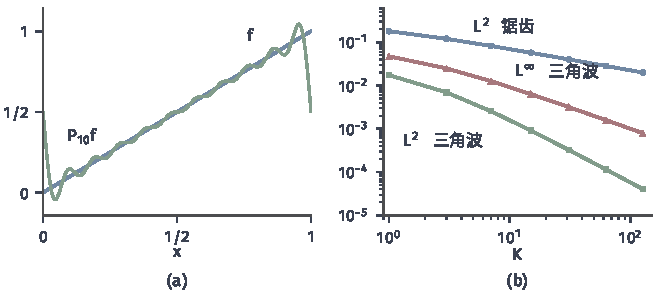
\includegraphics[width=112mm]{figures/04-spaces-measures-and-geometry/03-function-spaces/matplotlib/fapprox-fourier-truncation/figure.pdf}
  \caption{Fourier截断的误差。(a)锯齿函数$f(x)=x$（蓝）与截断$P_{10}f$（绿）。(b)误差随截断半径$K$的变化，双对数坐标，$K=1,3,7,\ldots,127$：锯齿函数的$L^2$误差按$K^{-1/2}$下降，三角波$\lvert x-\frac12\rvert$的$L^2$误差按$K^{-3/2}$下降，三角波的$L^\infty$误差按$K^{-1}$下降。}
  \label{fig:fapprox-fourier-truncation}
\end{BookInlineFigure}

\paragraph{理论截断与离散计算}
$P_Kf$中的系数是积分，实际计算时常用$M$个等距采样点上的求和代替：
\[
 \hat f_M(k)=\frac1M\sum_{j=0}^{M-1}f\Bigl(\frac jM\Bigr)\mathrm e^{-2\pi\mathrm ikj/M}.
\]
这相当于只读长向量上$M$个位置的分量，再用这$M$个数去估计频率坐标。$M$个数放不下无限多个频率坐标，必有信息被折叠到一起。

设系数绝对可和，在采样点使用连续代表$\tilde f=\sum_l\hat f(l)e_l$。把它代入上式，交换有限和与绝对收敛级数，内层出现的是几何和
\[
 \frac1M\sum_{j=0}^{M-1}\mathrm e^{2\pi\mathrm i(l-k)j/M}=
 \begin{cases}
  1,&l\equiv k\pmod M,\\
  0,&\text{其他情形}.
 \end{cases}
\]
于是
\begin{equation}
 \hat f_M(k)=\sum_{m\in\mathbb Z}\hat f(k+mM) .
 \label{eq:fapprox-aliasing}
\end{equation}
离散系数把所有与$k$模$M$同余的频率叠加在一起，这一现象称为\term{混叠}（aliasing）。

用三角波验证一下。取$M=4$，$k=1$，采样值依次是
\[
 f_*(0)=\frac12,\quad f_*\Bigl(\frac14\Bigr)=\frac14,\quad f_*\Bigl(\frac12\Bigr)=0,\quad f_*\Bigl(\frac34\Bigr)=\frac14 .
\]
指数因子依次是$1,-\mathrm i,-1,\mathrm i$，$j=1,3$两项相消，得到
\[
 \hat f_4(1)=\frac14\cdot\frac12=\frac18 .
\]

另一方面，$k+4m$取遍$\ldots,-7,-3,1,5,9,\ldots$，它们的绝对值恰好取遍所有正奇数各一次。由式~\eqref{eq:fapprox-aliasing}和$\sum_{n\ \text{奇},\,n>0}n^{-2}=\pi^2/8$，
\[
 \sum_{m\in\mathbb Z}\hat f_*(1+4m)=\frac1{\pi^2}\sum_{\substack{n>0\\n\ \text{奇}}}\frac1{n^2}=\frac18 ,
\]
两边相同。真实系数$\hat f_*(1)=1/\pi^2\approx0.1013$，被混入的高频抬高到了$0.125$。图~\ref{fig:fapprox-aliasing}(a)展示了混叠的机制，(b)展示了哪些频率被叠到一起。

\begin{BookInlineFigure}
  \centering
  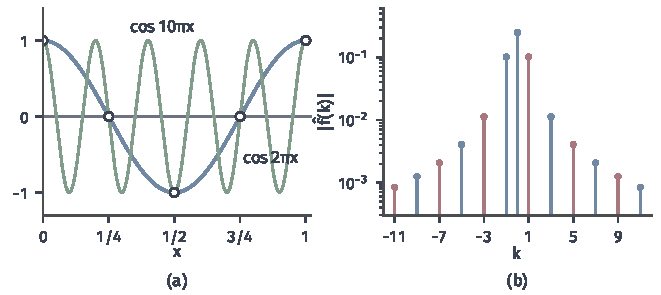
\includegraphics[width=112mm]{figures/04-spaces-measures-and-geometry/03-function-spaces/matplotlib/fapprox-aliasing/figure.pdf}
  \caption{$M=4$时的混叠。(a)$\cos2\pi x$（蓝）与$\cos10\pi x$（绿）在四个采样点$j/4$（空心圆）上取值相同，只看采样值无法区分频率$1$与$5$。(b)三角波系数的绝对值（对数纵轴）。红色频率$k\equiv1\pmod4$的系数相加，得到离散系数$\hat f_4(1)=1/8$；蓝色为其余频率。}
  \label{fig:fapprox-aliasing}
\end{BookInlineFigure}

用离散系数作截断时，误差有两个来源。设$g=\sum_{\lvert k\rvert\leq K}\hat f_M(k)e_k$，$f-g$分成互相正交的两部分：一部分在被舍弃的频率上，一部分在保留的频率上。勾股定理给出
\begin{equation}
 \lVert f-g\rVert_2^2=\sum_{\lvert k\rvert>K}\lvert\hat f(k)\rvert^2+\sum_{\lvert k\rvert\leq K}\lvert\hat f_M(k)-\hat f(k)\rvert^2 .
 \label{eq:fapprox-discrete-error}
\end{equation}

第一项是理论截断误差，只由$K$决定。第二项是离散误差，由式~\eqref{eq:fapprox-aliasing}知$\hat f_M(k)-\hat f(k)=\sum_{m\neq0}\hat f(k+mM)$，依赖采样数$M$与高频系数。两者应分别预算：增大$K$而不增大$M$，第二项不会减小；$2K+1>M$时，$M$个数据被重复计入不同的频率，增加保留项还会使离散误差变大。

\subsection{连续频带截断}
\label{sec:fapprox-band-truncation}

非周期函数没有离散频率，向量的“分量”换成了连续下标$\xi$上的$\hat f(\xi)$。相应的预算改为一段连续频带。在$L^2(\mathbb R)$上沿用第~\ref{chap:fourier-transform}章的归一化
\[
 \hat f(\xi)=\int_{\mathbb R}f(x)\mathrm e^{-2\pi\mathrm ix\xi}\,\mathrm dx ,
\]
先对$L^1\cap L^2$定义，再延拓到$L^2$。Plancherel等式是$\lVert\hat f\rVert_2=\lVert f\rVert_2$。

给定频带半宽$W>0$，令$Q_Wf$为$\hat f\mathbf 1_{[-W,W]}$的逆变换。乘以示性函数是$L^2$上的正交投影，Fourier变换是保持内积的双射，所以$Q_W$是到闭子空间
\[
 \mathcal B_W=\bigl\{g\in L^2(\mathbb R):\ \hat g=0\ \text{在}\ [-W,W]\ \text{外几乎处处成立}\bigr\}
\]
的正交投影。$\mathcal B_W$中的函数称为\term{带限函数}（band-limited function）。$Q_Wf$是$f$在$\mathcal B_W$中的最佳$L^2$逼近，由Plancherel等式，
\begin{equation}
 \lVert f-Q_Wf\rVert_2^2=\int_{\lvert\xi\rvert>W}\lvert\hat f(\xi)\rvert^2\,\mathrm d\xi .
 \label{eq:fapprox-band-tail}
\end{equation}

以Gauss函数$f(x)=\mathrm e^{-\pi x^2}$为例，$\hat f(\xi)=\mathrm e^{-\pi\xi^2}$。在积分区域上$\lvert\xi\rvert/W\geq1$，乘上这个因子可以把尾积分算出来：
\[
 \int_{\lvert\xi\rvert>W}\mathrm e^{-2\pi\xi^2}\,\mathrm d\xi\leq\frac2W\int_W^\infty\xi\,\mathrm e^{-2\pi\xi^2}\,\mathrm d\xi=\frac{\mathrm e^{-2\pi W^2}}{2\pi W}.
\]
$W=1$时误差$\lVert f-Q_Wf\rVert_2$约为$0.0167$，$W=1.5$时约为$2.7\times10^{-4}$。把右端的界开平方，分别得到$0.0172$与$2.8\times10^{-4}$，几乎与实际值一致。光滑而快速衰减的函数，频域尾部下降极快。

与上一小节比较，这里的预算是频带宽度而不是项数，而$\mathcal B_W$是无限维空间。例如，令$\operatorname{sinc}_W(x)=\sin(2\pi Wx)/(\pi x)$，$n\in\mathbb Z$，函数$\operatorname{sinc}_W(x-n/(2W))$的Fourier变换是
\[
 \mathbf 1_{[-W,W]}(\xi)\,\mathrm e^{-\pi\mathrm in\xi/W}.
\]
后者是区间$[-W,W]$上的Fourier基，彼此正交，所以这些函数在$\mathcal B_W$中两两正交，有无穷多个。频带截断去掉了高频，却没有把问题化为有限个参数；要进行有限计算，还需要进一步限制位置范围或在离散点上采样，这又带来新的截断误差与混叠误差。

\section{固定子空间的选择}
\label{sec:fapprox-fixed-subspaces}

最直接的有限表示，是在看到目标之前就选好一组方向或一张网格，再在它们张成的有限维子空间中找近似。这样的子空间对所有目标都一样，近似可以由少量取值或系数确定。本节在一致范数$\lVert f\rVert_\infty=\sup_x\lvert f(x)\rvert$下比较三种选法：全区间上的多项式、固定网格上的分段多项式，以及由一维表示组合出的多变量张量积。比较的量是维数、网格尺寸、目标的局部正则性，以及多变量时的总代价。

贯穿本节的目标是折线$f_*(x)=\lvert x-\frac12\rvert$，$x\in[0,1]$。它连续，却在$1/2$处有折点：多项式只能随次数增加而逼近它，而含结点$1/2$的分段线性函数能精确表示它。

\subsection{多项式逼近}
\label{sec:fapprox-polynomial}

次数至多$m$的多项式组成$m+1$维空间，次数就是表示预算。首先要问：在紧区间上，多项式能否一致逼近任意连续函数？下面构造一列具体的多项式来回答，并从构造中读出误差怎样依赖目标的正则性。

\paragraph{连续模}
要估计整个区间上的误差，需要一个量记录目标在小尺度上能变化多少。

\begin{definition}[连续模]
\label{def:fapprox-modulus}
设$f$是区间$I$上的有界函数。对$\delta>0$，令
\[
  \omega_f(\delta)=\sup\bigl\{\lvert f(s)-f(t)\rvert:\ s,t\in I,\ \lvert s-t\rvert\leq\delta\bigr\},
\]
称$\omega_f$为$f$的\term{连续模}（modulus of continuity）。
\end{definition}

连续模关于$\delta$单调不减。$f$在$I$上一致连续，恰好等价于$\delta\to0$时$\omega_f(\delta)\to0$；紧区间上的连续函数一致连续，所以$C[0,1]$中每个函数的连续模都趋于零。若$\lvert f(s)-f(t)\rvert\leq L\lvert s-t\rvert$，则$\omega_f(\delta)\leq L\delta$。对$f_*$，$\omega_{f_*}(\delta)=\min\{\delta,1/2\}$；对$\sqrt x$，由$\lvert\sqrt s-\sqrt t\rvert\leq\sqrt{\lvert s-t\rvert}$且在$s=0$处取等号，$\omega(\delta)=\sqrt\delta$（$\delta\leq1$），在原点附近变化得更剧烈。

\paragraph{Bernstein多项式}
固定$m\geq1$，在等距结点$j/m$处读取$f$的值，令
\begin{equation}
  B_mf(x)=\sum_{j=0}^{m}f\Bigl(\frac jm\Bigr)w_{m,j}(x),\qquad w_{m,j}(x)=\binom mjx^j(1-x)^{m-j},
  \label{eq:fapprox-bernstein}
\end{equation}
称为$f$的$m$次\term{Bernstein多项式}（Bernstein polynomial）。每个$w_{m,j}$是$m$次多项式，在$[0,1]$上非负，由二项式定理$\sum_jw_{m,j}(x)=(x+(1-x))^m=1$。所以$B_mf(x)$是结点值的凸组合。

凸组合本身还不说明$B_mf(x)$接近$f(x)$，还要知道权重集中在离$x$近的结点上。下面的矩恒等式把这一点写成精确的计算。

\begin{lemma}[Bernstein权重的矩]
\label{lem:fapprox-bernstein-moments}
对$0\leq x\leq1$与$m\geq1$，
\[
  \sum_{j=0}^mj\,w_{m,j}(x)=mx,\qquad \sum_{j=0}^mj(j-1)\,w_{m,j}(x)=m(m-1)x^2 ,
\]
从而
\begin{equation}
  \sum_{j=0}^m\Bigl(\frac jm-x\Bigr)^2w_{m,j}(x)=\frac{x(1-x)}m\leq\frac1{4m}.
  \label{eq:fapprox-bernstein-variance}
\end{equation}
\end{lemma}

\begin{proof}
由$j\binom mj=m\binom{m-1}{j-1}$，$j=0$的项为零，把下标改为$k=j-1$，
\[
  \sum_jj\,w_{m,j}(x)=mx\sum_{k=0}^{m-1}\binom{m-1}kx^k(1-x)^{m-1-k}=mx .
\]
第二式同理用$j(j-1)\binom mj=m(m-1)\binom{m-2}{j-2}$，$m=1$时两边为零。展开$(j/m-x)^2$并用$j^2=j(j-1)+j$，
\[
  \sum_j\Bigl(\frac jm-x\Bigr)^2w_{m,j}=\frac{m(m-1)x^2+mx}{m^2}-2x\cdot x+x^2=\frac{x(1-x)}m ,
\]
最后由$x(1-x)\leq1/4$得到上界。
\end{proof}

\begin{theorem}[Bernstein--Weierstrass逼近]
\label{thm:fapprox-bernstein}
设$f\in C[0,1]$。对每个$m\geq1$与$\delta>0$，
\begin{equation}
  \lVert B_mf-f\rVert_\infty\leq\omega_f(\delta)+\frac{\lVert f\rVert_\infty}{2m\delta^2}.
  \label{eq:fapprox-bernstein-error}
\end{equation}
因此$\lVert B_mf-f\rVert_\infty\to0$，多项式在$C[0,1]$中按一致范数稠密。
\end{theorem}

\begin{proof}
固定$x$。由权重和为一，$B_mf(x)-f(x)=\sum_j\bigl[f(j/m)-f(x)\bigr]w_{m,j}(x)$。把结点分成$\lvert j/m-x\rvert\leq\delta$的近邻组和其余的远处组。近邻组每个差值不超过$\omega_f(\delta)$，权重之和不超过$1$，贡献至多$\omega_f(\delta)$。远处组每个差值不超过$2\lVert f\rVert_\infty$，而在这些结点上$1<(j/m-x)^2/\delta^2$，由式~\eqref{eq:fapprox-bernstein-variance}，远处权重之和不超过$1/(4m\delta^2)$，贡献至多$\lVert f\rVert_\infty/(2m\delta^2)$。右端与$x$无关，取上确界即得式~\eqref{eq:fapprox-bernstein-error}。

为得到收敛，先由一致连续性选$\delta$使$\omega_f(\delta)<\varepsilon/2$，保持$\delta$不变，再取$m$足够大使第二项小于$\varepsilon/2$。次序不能颠倒：先固定$m$再缩小$\delta$，第二项会变大。
\end{proof}

这一结论称为\term{Weierstrass逼近定理}（Weierstrass approximation theorem），这里给出的是Bernstein的构造性证明\scite{bernstein1912demonstration}。经线性变量代换，它对任意紧区间成立。

\begin{figure}[!htb]
  \centering
  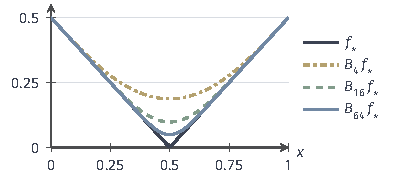
\includegraphics[width=66.7mm]{figures/02-abstract-mathematics/03-function-spaces/tikz/c6-bernstein-approx/figure.pdf}
  \caption{折线$f_*(x)=\lvert x-1/2\rvert$（黑）及其Bernstein多项式$B_4f_*$、$B_{16}f_*$、$B_{64}f_*$。每条曲线都是结点值的凸组合，位于$f_*$上方；一致误差都在$x=1/2$处取得，依次为$0.1875$、$0.0982$、$0.0497$，次数每增至四倍，误差约减半。}
  \label{fig:fapprox-bernstein}
\end{figure}

\paragraph{附加光滑性与误差速率}
定理保证$f_*$能被多项式任意逼近，但任何多项式都不等于$f_*$，因为多项式处处可微。“能任意逼近”与“给定次数下误差多大”是两个问题，后者需要对目标另加定量条件。若$f$是$L$-Lipschitz的，不必作近远分解，直接用Cauchy--Schwarz不等式与式~\eqref{eq:fapprox-bernstein-variance}：
\[
  \lvert B_mf(x)-f(x)\rvert\leq L\sum_j\Bigl\lvert\frac jm-x\Bigr\rvert w_{m,j}(x)\leq L\Bigl(\sum_j\Bigl(\frac jm-x\Bigr)^2w_{m,j}(x)\Bigr)^{1/2}\leq\frac L{2\sqrt m}.
\]
对$f_*$，$L=1$，界在$m=4,16,64$时为$0.25$、$0.125$、$0.0625$，与图~\ref{fig:fapprox-bernstein}中的实际误差同阶。对$\sqrt x$只有$\lvert f(s)-f(t)\rvert\leq\lvert s-t\rvert^{1/2}$，同样的论证（先对$\lvert j/m-x\rvert^{1/2}$用Cauchy--Schwarz）只给出$(4m)^{-1/4}$。条件越弱，这一构造能保证的速率越慢。

更多的光滑性并不能让Bernstein多项式更快。由引理~\ref{lem:fapprox-bernstein-moments}，$B_m(x^2)=x^2+x(1-x)/m$，误差恰为$1/(4m)$量级，而$x^2$本身就是二次多项式，$m\geq2$时最佳误差为零。所以Bernstein构造给出的是对所有连续函数都可验证的收敛机制，不是给定次数下的最佳近似。对最佳多项式逼近误差$E_m(f)=E(f,\mathcal P_m)_\infty$，其中$\mathcal P_m$是次数至多$m$的多项式空间，Jackson型定理给出：若$f\in C^r[a,b]$，则$E_m(f)\leq C_rm^{-r}\omega_{f^{(r)}}(1/m)$，常数$C_r$只依赖$r$与区间。光滑性越高，最佳多项式误差下降越快；对只有折点的$f_*$，最佳误差按$1/m$下降，也不能更快。这两条结论这里都不给出证明。

多项式还有一个结构上的特点：它是全局的。改变一个系数，整个区间上的函数值都会改变；Bernstein权重也在整个$(0,1)$上非零。目标若只在一处不光滑，例如$f_*$的折点，这一处的困难会影响全区间上的近似。下一小节的分段表示把这种影响限制在局部。

\subsection{固定网格上的分段逼近}
\label{sec:fapprox-fixed-grid}

另一种思路是先把区间切成小段，每段只用低次多项式。固定结点$0=t_0<t_1<\cdots<t_N=1$，记网格尺寸$h=\max_i(t_{i+1}-t_i)$。网格在看到目标之前就已经选定，所以候选集合仍是固定的线性空间；预算由单元数$N$和每个单元内的次数共同决定。

\paragraph{分段常数与分段多项式}
最简单的选择是每个单元上取常数。若在单元$[t_i,t_{i+1}]$上取该单元内函数值的最佳常数$(\max+\min)/2$，由第~\ref{sec:fapprox-fixed-space}节，单元上的误差为振幅的一半，因此整体一致误差不超过$\omega_f(h)/2$。若$f\in C^1$，振幅不超过$h\lVert f'\rVert_\infty$，误差至多$h\lVert f'\rVert_\infty/2$，按一阶下降。

每个单元上用$r$次多项式、单元之间不加任何衔接条件时，空间维数为$N(r+1)$。若$f\in C^{r+1}[0,1]$，在每个单元上取$f$在中点$c_i$处的$r$次Taylor多项式，由Taylor余项，单元内
\[
  \lvert f(x)-p_i(x)\rvert\leq\frac{\lVert f^{(r+1)}\rVert_\infty}{(r+1)!}\Bigl(\frac h2\Bigr)^{r+1}.
\]
误差按$h^{r+1}$下降。这是一个可验证的构造，不必是该空间中的最佳近似；它说明提高单元内次数换来的是更高的阶，前提是目标有相应阶的有界导数。

\paragraph{分段线性插值}
在实际中更常用的是连续的分段线性函数。对$x\in[t_i,t_{i+1}]$，令
\begin{equation}
  S_hf(x)=(1-s)f(t_i)+s\,f(t_{i+1}),\qquad s=\frac{x-t_i}{t_{i+1}-t_i}\in[0,1].
  \label{eq:fapprox-linear-interpolant}
\end{equation}
相邻两段在公共结点取同一个值，所以$S_hf$是经过全部结点值的连续折线，称为$f$的\term{分段线性插值}（piecewise linear interpolation）。在每段上为一次函数的全体连续函数组成$N+1$维空间。对每个结点$t_i$，令$\varphi_i$为在$t_i$处取$1$、在其余结点取$0$的连续折线，它在$[t_{i-1},t_{i+1}]$上呈三角形，称为\term{帽形函数}（hat function）。于是$S_hf=\sum_if(t_i)\varphi_i$，系数就是结点值。

\begin{theorem}[分段线性插值的误差]
\label{thm:fapprox-linear-interpolation}
若$f\in C[0,1]$，则$\lVert f-S_hf\rVert_\infty\leq\omega_f(h)$。若进一步$f\in C^2[0,1]$，则
\begin{equation}
  \lVert f-S_hf\rVert_\infty\leq\frac{h^2}8\lVert f''\rVert_\infty .
  \label{eq:fapprox-interpolation-quadratic}
\end{equation}
\end{theorem}

\begin{proof}
在单元$[t_i,t_{i+1}]$上，$f(x)-S_hf(x)=(1-s)\bigl(f(x)-f(t_i)\bigr)+s\bigl(f(x)-f(t_{i+1})\bigr)$。$x$到两端点的距离都不超过$h$，两个差值都不超过$\omega_f(h)$，凸组合也不超过$\omega_f(h)$。

再证二阶界。固定单元内一点$x\in(t_i,t_{i+1})$，令$g=f-S_hf$，它在两端为零。取
\[
  \kappa=\frac{g(x)}{(x-t_i)(x-t_{i+1})},\qquad G(u)=g(u)-\kappa(u-t_i)(u-t_{i+1}),
\]
则$G$在$t_i,x,t_{i+1}$三点为零。两次使用Rolle定理，存在$\xi$使$G''(\xi)=0$。$S_hf$在单元内是一次函数，$G''(\xi)=f''(\xi)-2\kappa$，故
\[
  f(x)-S_hf(x)=\frac{f''(\xi)}2(x-t_i)(x-t_{i+1}).
\]
单元上$\lvert(x-t_i)(x-t_{i+1})\rvert\leq(t_{i+1}-t_i)^2/4\leq h^2/4$，代入即得。
\end{proof}

两个界依据不同。连续模界只用了凸组合，对任何连续目标都成立，也不要求等距：只要网格尺寸$h\to0$，插值就一致收敛。二阶界多用了$f''$的有界性，换来$h^2$的速率。常数$1/8$不能改进：取$f(x)=x^2$与两个结点$0,1$，误差$x-x^2$在$1/2$处取到$1/4=h^2\lVert f''\rVert_\infty/8$。

\paragraph{局部正则性与网格位置}
二阶速率所需的光滑性不能省略。取等距结点$t_i=i/N$，$N$为奇数，此时$1/2$不是结点，而是某个单元的中点。$f_*$在这个单元两端的值都是$h/2$，插值在单元内恒为$h/2$，而$f_*(1/2)=0$；其余单元上$f_*$本身是直线，插值没有误差。所以$\lVert f_*-S_hf_*\rVert_\infty=h/2$，只按一阶下降。图~\ref{fig:fapprox-spline-rates}在对数坐标中比较了光滑目标$\sin(\pi x)$与$f_*$：前者的误差贴近二阶界，后者恰为$h/2$。

\begin{figure}[!htb]
  \centering
  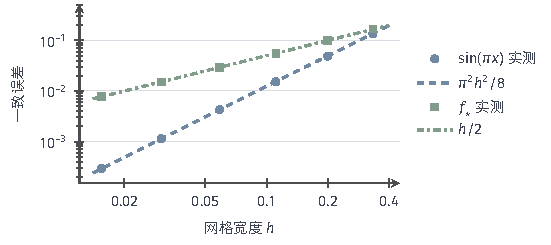
\includegraphics[width=93.4mm]{figures/02-abstract-mathematics/03-function-spaces/tikz/c6-spline-rates/figure.pdf}
  \caption{等距线性插值的一致误差与网格宽度$h=1/N$（$N=3,5,\ldots,65$为奇数，$1/2$不是结点），双对数坐标。光滑目标$\sin(\pi x)$的误差（圆点）贴近二阶界$\pi^2h^2/8$；折线$f_*$的误差（方块）恰为$h/2$，只按一阶下降。}
  \label{fig:fapprox-spline-rates}
\end{figure}

反过来，若结点恰好包含$1/2$，$f_*$在每个单元上都是直线，插值没有误差；用$t_0=0,t_1=1/2,t_2=1$三个结点就有$f_*=\frac12\varphi_0+0\cdot\varphi_1+\frac12\varphi_2$。同一个固定网格空间，对有的目标很有效，对稍微挪动了折点位置的目标就只剩一阶速率。固定网格的误差由目标在每个单元内的局部正则性决定，而折点落在哪个单元，在选网格时并不知道。这正是第~\ref{sec:fapprox-adaptive}节让分点随目标移动的动机。

\paragraph{拼接条件与维数}
单元之间的衔接条件改变维数，但不改变上面的阶。$N$个单元上不衔接的分段线性函数有$2N$维，要求连续后减少$N-1$个自由度，剩下$N+1$维，误差阶仍为$h^2$。更一般地，每段为$k$次多项式、在内部结点处$k-1$阶导数连续的函数称为$k$次\term{样条}（spline）。$N$段各有$k+1$个系数，$N-1$个内部结点各施加$k$个条件，维数为$(k+1)N-k(N-1)=N+k$；常用的三次样条维数为$N+3$。衔接条件让近似更光滑，并以较少的参数达到同样的阶，代价是系数与结点值不再一一对应，插值需要解一个线性方程组。

\paragraph{与全局多项式的比较}
在相同维数下比较两类空间。对光滑目标，维数为$N+1$的分段线性插值误差按$N^{-2}$下降，而次数为$N$的最佳多项式误差按Jackson型估计可以下降得更快；对$f_*$这类只在一点不光滑的目标，两者都只有一阶速率，但分段插值的误差只集中在含折点的一个单元里，其余单元上没有误差。全局多项式利用整体光滑性，分段多项式利用局部光滑性。选择哪一种，取决于目标的光滑性是整体的还是局部的。

\subsection{张量积表示}
\label{sec:fapprox-tensor}

目标有多个变量时，最自然的固定子空间是由一维表示相乘得到的。给定$x$方向的函数$\varphi_1,\ldots,\varphi_m$与$y$方向的函数$\psi_1,\ldots,\psi_n$，乘积$(\varphi_i\otimes\psi_k)(x,y)=\varphi_i(x)\psi_k(y)$称为两者的\term{张量积}（tensor product）。全体乘积的线性组合组成$mn$维空间（每组函数线性无关时），系数排成$m\times n$矩阵；有限维的张量积与Kronecker积可参考\BookChapterRef{chap:linear-operations}{卷二第1章“向量、矩阵与张量的运算”}。

\paragraph{网格插值与组合误差}
在$[0,1]$上取等距结点$t_i=i/(m-1)$，$i=0,\ldots,m-1$，帽形函数为$\varphi_0,\ldots,\varphi_{m-1}$，网格宽度$h=1/(m-1)$。二维插值取
\[
  (\Pi f)(x,y)=\sum_{i=0}^{m-1}\sum_{k=0}^{m-1}f(t_i,t_k)\,\varphi_i(x)\varphi_k(y).
\]
乘积$\varphi_i\otimes\varphi_k$支撑在一个矩形上，任一点只受它所在网格单元四个角点的影响，这就是双线性插值。图~\ref{fig:fapprox-tensor-grid}(a)画出$m=5$时一个乘积基的支撑与一个查询点所用的四个角点。

误差可以由一维结果逐个方向得到，但要多用一条性质。记$I_x$为固定$y$只对$x$作线性插值，$I_y$类似，则$\Pi=I_xI_y$。$I_x$是结点值的凸组合，所以$\lVert I_xg\rVert_\infty\leq\lVert g\rVert_\infty$。若$f\in C^2([0,1]^2)$，由定理~\ref{thm:fapprox-linear-interpolation}，
\[
  \lVert f-\Pi f\rVert_\infty\leq\lVert f-I_xf\rVert_\infty+\lVert I_x(f-I_yf)\rVert_\infty\leq\frac{h^2}8\bigl(\lVert\partial_x^2f\rVert_\infty+\lVert\partial_y^2f\rVert_\infty\bigr).
\]
第二项能用一维误差控制，靠的是$I_x$不放大一致范数；若某个方向的插值算子范数大于$1$，组合后的整体误差会被这个范数放大，单变量误差就不足以控制它。同样的论证在$d$维给出误差至多$d\,h^2\max_i\lVert\partial_i^2f\rVert_\infty/8$。

\paragraph{成本随维数的增长}
误差只随维数线性增大，所需系数个数却是$m^d$。设每个$\lVert\partial_i^2f\rVert_\infty\leq1$，要求误差不超过$\varepsilon=10^{-3}$，上式要求$h^2\leq8\varepsilon/d$。$d=2$时$h\leq0.0632$，取$m=17$，共$289$个系数；$d=6$时$h\leq0.0365$，需要$m=29$，共$29^6\approx5.9\times10^8$个系数。每个方向的分辨率只略有提高，总数却增长了六个数量级。这种由完整组合造成的规模增长称为\term{维数灾难}（curse of dimensionality）。第~\ref{sec:fapprox-fourier-truncation}节的多变量Fourier截断有同样的现象：保留$\max_i\lvert k_i\rvert\leq K$需要$(2K+1)^d$个系数。

\begin{figure}[!htb]
  \centering
  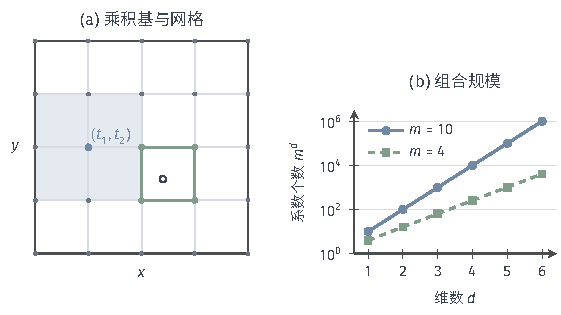
\includegraphics[width=95.0mm]{figures/02-abstract-mathematics/03-function-spaces/tikz/c6-tensor-grid/figure.pdf}
  \caption{张量积网格。(a)每轴$m=5$个结点，蓝底为乘积帽形基$\varphi_1(x)\varphi_2(y)$的支撑，蓝点为其中心结点$(t_1,t_2)$；空心圆为一个查询点，双线性插值只用它所在单元的四个角点（绿）。(b)完整张量积系数个数$m^d$随维数$d$指数增长（对数纵轴）。}
  \label{fig:fapprox-tensor-grid}
\end{figure}

比较成本时要写明计数的对象。上面数的是需要存储的系数，也就是网格上的函数值个数$m^d$；在一个点上求值只用所在单元的$2^d$个角点，代价随维数增长得慢得多；而确定这些系数需要的函数取样次数又与系数个数相同。“维数灾难”指的是前一种计数在固定误差要求下的指数增长，它来自对每个方向都使用同样分辨率的完整组合，并不说明所有多变量逼近都必须付出这样的代价。

\section{最佳N项逼近}
\label{sec:fapprox-best-n-term}

固定子空间对所有目标一视同仁：截断Fourier级数总是保留低频，固定网格总是在同样的位置细分。目标的重要信息若集中在少数几个预先没有选中的方向上，固定选法就会浪费预算。本节仍固定一组完备标准正交基，但允许根据目标挑选保留哪些基向量，只限制挑选的个数。

先用一个向量看这件事。在$\mathbb R^5$中取
\[
 v=(0.1,\ 3,\ -0.2,\ 2,\ 0.4).
\]
若只能留两个坐标，总是留前两个的话，被舍弃的是$-0.2,2,0.4$，平方误差是$0.04+4+0.16=4.2$。若留绝对值最大的两个，即$3$和$2$，被舍弃的是$0.1,-0.2,0.4$，平方误差只有$0.21$。同样的预算，差了二十倍。

设$H$是可分Hilbert空间，$(e_n)_{n\geq1}$是一组标准正交基，$f$的系数为$c_n=\langle e_n,f\rangle$。对预算$N$，令
\[
 \Sigma_N=\Bigl\{\sum_{n\in\Lambda}a_ne_n:\ \Lambda\subseteq\mathbb N,\ \lvert\Lambda\rvert\leq N,\ a_n\in\mathbb K\Bigr\}.
\]

\begin{definition}[最佳N项逼近]
\label{def:fapprox-best-n-term}
称
\begin{equation}
 \sigma_N(f)_2=E(f,\Sigma_N)_H=\inf_{g\in\Sigma_N}\lVert f-g\rVert
 \label{eq:fapprox-best-n-term}
\end{equation}
为$f$关于基$(e_n)$的最佳$N$项误差；达到这个下确界的元素称为$f$的\term{最佳N项逼近}（best N-term approximation）。
\end{definition}

$\Sigma_N$是第~\ref{sec:fapprox-budget}节所说的非线性候选集合。它是所有至多$N$维坐标子空间的并，两个元素之和可能用到$2N$个基向量；图~\ref{fig:fapprox-nearest-point}(c)画的正是$\mathbb R^2$中的$\Sigma_1$。非线性只来自支撑集合$\Lambda$依赖于目标，一旦$\Lambda$选定，近似就是在线性子空间$\operatorname{span}\{e_n:n\in\Lambda\}$中作正交投影。

\subsection{固定截断与自适应选择}
\label{sec:fapprox-fixed-vs-adaptive}

在同一组基和同一个项数下比较两种做法。固定截断预先规定下标集合$\Lambda_N=\{1,\ldots,N\}$，对所有目标都保留前$N$项，误差为
\[
 \Bigl(\sum_{n>N}\lvert c_n\rvert^2\Bigr)^{1/2},
\]
这是第~\ref{sec:fapprox-fixed-space}节在$V_N=\operatorname{span}\{e_1,\ldots,e_N\}$中的最佳逼近。自适应选择则对每个目标分别挑选$\Lambda$。由定义，$\sigma_N(f)_2$不超过固定截断的误差，差距取决于大系数是否恰好排在前面。

极端情形下差距可以达到最大。取$f=e_{N+1}$，固定截断的误差为$\lVert f\rVert=1$，而一项就能精确表示它，$\sigma_1(f)_2=0$。不那么极端的情形同样常见：一个大部分区域光滑、只在某处有跳跃的函数，在小波基中的大系数集中在跳跃附近的细尺度上，按“先粗后细、从左到右”的固定次序要保留许多无用的系数才能轮到它们。

自适应选择的代价是需要知道系数的大小。要挑出重要的系数，通常得先计算或估计足够多的系数，再按大小筛选；被挑出的下标集合也要存储，它本身就是表示的一部分。所以最佳$N$项误差衡量的是“已知全部系数时用$N$项能做到多好”，它与在有限计算下找到这些项的问题是两回事。

\subsection{最大系数选择}
\label{sec:fapprox-largest-coefficients}

在正交基和$L^2$型范数下，最佳$N$项逼近有简单的显式解。由$f\in H$，$\sum_n\lvert c_n\rvert^2<\infty$，所以对任意$t>0$，满足$\lvert c_n\rvert\geq t$的下标只有有限个。于是可以把系数的绝对值按非增次序排列为
\[
 c_1^*\geq c_2^*\geq\cdots
\]
相等的值任意排序，非零系数有限时在末尾补零。

\begin{theorem}[保留最大系数最优]
\label{thm:fapprox-largest-coefficients}
设$\Lambda_N^*$是$\lvert c_n\rvert$最大的$N$个下标组成的集合，$g_N=\sum_{n\in\Lambda_N^*}c_ne_n$。则$g_N$是$f$的最佳$N$项逼近，并且
\begin{equation}
 \sigma_N(f)_2^2=\sum_{n>N}(c_n^*)^2 .
 \label{eq:fapprox-largest-coefficients}
\end{equation}
\end{theorem}

\begin{proof}
任取$\lvert\Lambda\rvert\leq N$与系数$a_n$，令$g=\sum_{n\in\Lambda}a_ne_n$。由Parseval等式，$f-g$的平方范数按坐标拆开：
\[
 \lVert f-g\rVert^2=\sum_{n\in\Lambda}\lvert c_n-a_n\rvert^2+\sum_{n\notin\Lambda}\lvert c_n\rvert^2 .
\]
第一项非负，在$a_n=c_n$时为零。所以对固定的$\Lambda$，最好的系数就是原系数，于是
\[
 \lVert f-g\rVert^2\geq\sum_{n\notin\Lambda}\lvert c_n\rvert^2=\lVert f\rVert^2-\sum_{n\in\Lambda}\lvert c_n\rvert^2 .
\]

$\Lambda$至多含$N$个下标，$\sum_{n\in\Lambda}\lvert c_n\rvert^2$不超过最大的$N$个平方之和，等号在$\Lambda=\Lambda_N^*$时取到。所以
\[
 \lVert f-g\rVert^2\geq\lVert f\rVert^2-\sum_{n\leq N}(c_n^*)^2=\sum_{n>N}(c_n^*)^2 ,
\]
而$g_N$达到这个下界。
\end{proof}

证明依赖两件事。第一，误差平方能拆成各方向上的平方和，这来自基的正交性和Parseval等式。第二，这种拆分让“选哪些方向”与“选什么系数”分开处理。若基不正交，或使用冗余的字典，同一个函数有多种展开，系数本身不唯一，误差也不再是舍弃系数的平方和。

换一把尺子同样会出问题。用下面的Haar基，取$f=1.2\varphi+\psi_{2,0}$，一致范数下比较保留哪一项。$\psi_{2,0}$在$[0,\frac18)$上取$2$、在$[\frac18,\frac14)$上取$-2$，其余为零。按最大系数规则保留系数$1.2$的$\varphi$，则对任何$a$，$f-a\varphi$在这两段上相差$4$，所以
\[
 \lVert f-a\varphi\rVert_\infty\geq2 .
\]
改为保留系数较小的$\psi_{2,0}$，误差只有$\lVert1.2\varphi\rVert_\infty=1.2$。原因是细尺度的基函数高而窄，系数小但一致范数大。

\paragraph{Haar展开中的选择}
用第~\ref{chap:wavelet-transform}章的Haar基复算这一选择。在$L^2(0,1)$上，记
\[
 \varphi=\mathbf 1_{[0,1)},\qquad \psi=\mathbf 1_{[0,1/2)}-\mathbf 1_{[1/2,1)},\qquad \psi_{j,k}(x)=2^{j/2}\psi(2^jx-k),
\]
其中$j\geq0$，$0\leq k<2^j$；$\varphi$与全体$\psi_{j,k}$组成标准正交基。取在$3/4$处向下跳跃的阶梯函数
\[
 f=3\cdot\mathbf 1_{[0,3/4)}-\mathbf 1_{[3/4,1)} .
\]

逐个计算内积。$\varphi$的系数就是平均值：
\[
 \langle\varphi,f\rangle=\frac{3\cdot3-1}4=2 .
\]
$\psi_{0,0}$的系数是左半积分减右半积分：
\[
 \langle\psi_{0,0},f\rangle=\int_0^{1/2}f-\int_{1/2}^1f=\frac32-\frac12=1 .
\]
下一层的两个系数分别是
\[
 \langle\psi_{1,0},f\rangle=0,\qquad
 \langle\psi_{1,1},f\rangle=\sqrt2\Bigl(\int_{1/2}^{3/4}f-\int_{3/4}^1f\Bigr)=\sqrt2 .
\]
$j\geq2$时，$\psi_{j,k}$支撑在某个长为$1/4$的二进区间内且积分为零，$f$在这样的区间上是常数，内积为零。

于是$f$只有三个非零坐标：
\[
 f=2\varphi+\psi_{0,0}+\sqrt2\,\psi_{1,1}.
\]
用Parseval等式检验：$\lVert f\rVert^2=(9\cdot3+1)/4=7$，而$2^2+1^2+(\sqrt2)^2=7$。

按“先粗后细、同层从左到右”的固定次序$\varphi,\psi_{0,0},\psi_{1,0},\psi_{1,1},\ldots$截断，保留两项得$2\varphi+\psi_{0,0}$，误差平方为$2$；保留三项仍缺$\psi_{1,1}$，误差平方仍为$2$。系数绝对值的非增排列是$2,\sqrt2,1,0,\ldots$，由定理~\ref{thm:fapprox-largest-coefficients}，最佳两项逼近为$2\varphi+\sqrt2\,\psi_{1,1}$，误差平方为
\[
 \sigma_2(f)_2^2=1 .
\]
最佳三项逼近就是$f$本身，$\sigma_3(f)_2=0$。

图~\ref{fig:fapprox-best-n-term}对照了两种选择。固定次序的近似在跳跃所在的右半区间上偏差最大；最佳两项逼近把预算用到了$\psi_{1,1}$，正好捕捉到跳跃，代价是在左半区间留下幅度为$1$的偏差。跳跃位于右半区间的细尺度上，固定次序先用掉了左半区间那个为零的系数，自适应选择直接找到了它。

\begin{BookInlineFigure}
  \centering
  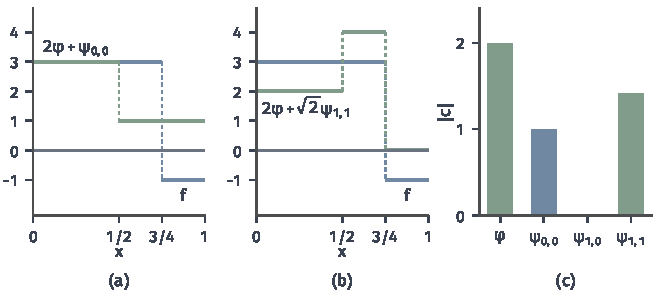
\includegraphics[width=112mm]{figures/04-spaces-measures-and-geometry/03-function-spaces/matplotlib/fapprox-best-n-term/figure.pdf}
  \caption{同一预算下的两种选择。目标$f$（蓝）在$3/4$处跳跃，均保留两项（绿）。(a)固定次序保留$\varphi,\psi_{0,0}$，误差平方为$2$。(b)保留系数最大的$\varphi,\psi_{1,1}$，误差平方为$1$。(c)前四个Haar系数的绝对值，绿色为最佳两项选中的系数；固定次序选的是前两根柱子。}
  \label{fig:fapprox-best-n-term}
\end{BookInlineFigure}

\section{自适应分段逼近}
\label{sec:fapprox-adaptive}

第~\ref{sec:fapprox-fixed-grid}节的固定网格在看到目标之前就选定了分点，误差由目标在最差单元上的局部正则性决定。若目标只在少数地方变化剧烈，更合理的做法是在那里多放分点，在平缓处少放。上一节只调整“留哪几个坐标”，这里连坐标轴本身也按目标调整：分点就是把长向量的下标切成几段的位置。

本节把预算固定为区间个数$N$，允许分点随目标移动，在一致范数下比较固定网格与自适应分割，并区分三个问题：最佳分割是否存在，它的误差有多大，以及怎样找到一个好的分割。

\paragraph{候选集合与局部误差}
在$[0,1]$上，令$\mathcal S_N$为全体至多$N$段的分段常数函数：存在$0=x_0\leq x_1\leq\cdots\leq x_N=1$，函数在每个$[x_{i-1},x_i)$上为常数，最后一段含右端点。分点是候选的一部分，所以$\mathcal S_N$不是线性空间，相应的逼近称为\term{自适应分段逼近}（adaptive piecewise approximation）。

分割固定后，每段上的最佳常数由式~\eqref{eq:fapprox-best-constant}给出：在$I=[a,b]$上，局部误差是振幅的一半，记为$\frac12\operatorname{osc}(f,I)$，其中$\operatorname{osc}(f,I)=\max_If-\min_If$。所以对连续的$f$，
\begin{equation}
 E(f,\mathcal S_N)_\infty=\frac12\inf_{0=x_0\leq\cdots\leq x_N=1}\ \max_{1\leq i\leq N}\operatorname{osc}\bigl(f,[x_{i-1},x_i]\bigr).
 \label{eq:fapprox-adaptive-error}
\end{equation}
寻找最佳逼近化成了一个只关于分点的问题：让最大的局部振幅尽可能小。

\paragraph{平方根函数的比较}
以$f(x)=\sqrt x$为例。它在$[0,1]$上连续递增，但在原点附近导数无界，不是Lipschitz的。等距网格$x_i=i/N$上，单元$[x_{i-1},x_i]$的振幅是
\[
 \sqrt{\frac iN}-\sqrt{\frac{i-1}N},
\]
随$i$递减，最大的是第一个单元的$\sqrt{1/N}$。所以固定网格的误差为
\[
 \frac1{2\sqrt N}.
\]

若改取$x_i=(i/N)^2$，每个单元的振幅都是
\[
 \sqrt{x_i}-\sqrt{x_{i-1}}=\frac1N ,
\]
误差为$1/(2N)$。$N=100$时，前者为$0.05$，后者为$0.005$。分点向原点聚集，把局部误差平均分配到各个单元。图~\ref{fig:fapprox-adaptive}(a)(b)画出$N=6$的两种分割。

这个分割还是最优的。任一分割的各段振幅之和为
\[
 \sum_i\bigl(\sqrt{x_i}-\sqrt{x_{i-1}}\bigr)=1 ,
\]
$N$个数之和为$1$，最大者不小于$1/N$。所以$E(\sqrt{\cdot},\mathcal S_N)_\infty=1/(2N)$，自适应分段把速率从$N^{-1/2}$提高到$N^{-1}$，而固定网格要达到同样的速率需要目标是Lipschitz的。

\begin{BookInlineFigure}
  \centering
  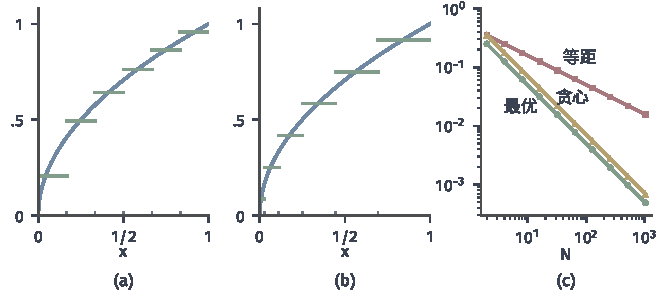
\includegraphics[width=112mm]{figures/04-spaces-measures-and-geometry/03-function-spaces/matplotlib/fapprox-adaptive/figure.pdf}
  \caption{$\sqrt x$的分段常数逼近，每段取最佳常数（绿），下方刻线为分点。(a)$N=6$的等距分割，误差集中在第一段。(b)$N=6$的分割$x_i=(i/6)^2$，每段振幅相同。(c)一致误差随段数$N$的变化，双对数坐标：等距为$1/(2\sqrt N)$，最优为$1/(2N)$，二进贪心细分的误差约为最优的$\sqrt2$倍。}
  \label{fig:fapprox-adaptive}
\end{BookInlineFigure}

\paragraph{单调函数的误差界}
平方根例子中用到的只是单调性，并不需要可微。把振幅之和等于总变化量的论证写成一般形式，就得到下面的结论。

\begin{theorem}[单调函数的自适应分段误差]
\label{thm:fapprox-monotone}
设$f$在$[a,b]$上连续且单调，$V=\lvert f(b)-f(a)\rvert$。则
\begin{equation}
 E(f,\mathcal S_N)_\infty=\frac V{2N},
 \label{eq:fapprox-monotone}
\end{equation}
并且存在达到这一误差的分割。
\end{theorem}

\begin{proof}
不妨设$f$不减。对任一分割，各段振幅为$f(x_i)-f(x_{i-1})$，其和为$V$，最大者不小于$V/N$，所以误差不小于$V/(2N)$。

反过来，令$x_0=a$，对$i=1,\ldots,N$取
\[
 x_i=\min\Bigl\{x\in[a,b]:\ f(x)=f(a)+\frac{iV}N\Bigr\}.
\]
由介值定理这样的点存在，由连续性最小值能取到，水平递增时这些点不减。$x_N\leq b$，把最后一个分点改成$b$，$f$在多出的一段上恒为$f(b)$，不改变取值范围。

在$[x_{i-1},x_i]$上，$f$的取值落在$f(a)+(i-1)V/N$与$f(a)+iV/N$之间，振幅不超过$V/N$。由式~\eqref{eq:fapprox-adaptive-error}，误差不超过$V/(2N)$。
\end{proof}

定理把误差与总变化量$V$联系起来，而不是与导数或连续模联系。固定网格的误差由$\omega_f(h)$控制，要求处处都不能变化太快；自适应分割只要求变化的总量有限，变化集中在哪里都可以。在同一预算和同一误差范数下，两种候选集合对目标正则性的要求不同。

\paragraph{最佳分割的存在}
对一般的连续函数，最佳分割同样存在，但通常没有显式公式。分点向量$(x_1,\ldots,x_{N-1})$在紧集$\{0\leq x_1\leq\cdots\leq x_{N-1}\leq1\}$中变化。由$f$一致连续，$\operatorname{osc}(f,[a,b])$是$(a,b)$的连续函数：端点移动不超过$\eta$时，最大值与最小值各自至多改变$\omega_f(\eta)$。

所以最大局部振幅是分点的连续函数，在紧集上取到最小值。允许相邻分点重合，相当于允许少于$N$段，并不改变$\mathcal S_N$。这一论证和第~\ref{sec:fapprox-fixed-space}节的存在定理一样靠紧性，只是紧的集合从有限维子空间中的闭球换成了分点的单纯形。

存在性与误差界是两回事。存在性论证没有说明最佳误差有多大，也没有给出找到最佳分割的方法；单调函数的定理给出了误差的精确值，构造却依赖于知道$f$的水平集位置。

\paragraph{贪心细分}
实际中常用的是一种简单的算法：从整个区间出发，每一步找出局部误差最大的单元，把它从中点一分为二，直到用完$N$个单元。每步只需计算新产生的两个单元的振幅，分点都落在二进点上。

用$\sqrt x$跑前几步。第一步把$[0,1]$对半切，两段的振幅是
\[
 \operatorname{osc}\bigl(\sqrt{\cdot},[0,\tfrac12]\bigr)=0.7071,\qquad
 \operatorname{osc}\bigl(\sqrt{\cdot},[\tfrac12,1]\bigr)=0.2929 .
\]
第二步切振幅最大的$[0,\frac12]$，得到$[0,\frac14]$的振幅$0.5$和$[\frac14,\frac12]$的振幅$0.2071$。第三步切$[0,\frac14]$，得到振幅$0.3536$和$0.1464$。

这时四个单元从左到右的振幅是
\[
 0.3536,\quad 0.1464,\quad 0.2071,\quad 0.2929 .
\]
最大误差是$0.3536/2=0.1768$，而$N=4$的最优误差是$1/8=0.125$。贪心细分总是先切靠近原点的单元，却只能对半切，各单元的振幅不能像最优分割那样恰好相等。

表~\ref{tab:fapprox-greedy}列出了几种$N$的结果。这个例子中贪心误差始终是最优误差的约$\sqrt2$倍，也就是说，它达到了与最优分割相同的速率$N^{-1}$，只损失一个常数。这是对$\sqrt x$的计算观察，不是一般定理；贪心细分与最佳误差的比较需要针对目标类另作分析。

\begin{BookInlineTable}
  \centering
  \caption{$\sqrt x$的分段常数逼近的一致误差}
  \label{tab:fapprox-greedy}
  \begin{tabular}{rlll}
    \toprule
    $N$ & 等距$1/(2\sqrt N)$ & 贪心细分 & 最优$1/(2N)$ \\
    \midrule
    $4$ & $0.25$ & $0.1768$ & $0.125$ \\
    $16$ & $0.125$ & $0.0442$ & $0.0313$ \\
    $64$ & $0.0625$ & $0.0110$ & $0.0078$ \\
    $1024$ & $0.0156$ & $0.00069$ & $0.00049$ \\
    \bottomrule
  \end{tabular}
\end{BookInlineTable}

二进的贪心细分与上一节的Haar展开密切相关：在二进区间上保留或舍去细分，相当于在Haar展开中保留或舍去对应的细节系数。哪些函数能被这样的自适应表示以给定速率逼近，可以用函数在不同尺度上的局部变化来刻画，这正是第~\ref{chap:besov-spaces}章研究的问题。

\section{本章小结}
\label{sec:fapprox-summary}

本章开头问：哪些简单函数能以任意精度逼近目标，加入表示预算后最佳误差又怎样随预算变化。对第一个问题，答案依赖测度、积分指数与误差范数。在任意测度空间中，截断与二进分层的简单函数在$L^p$（$1\leq p<\infty$）中稠密；在Lebesgue区域上，有理矩形与有理复系数给出可数稠密族，$L^p$可分，一般测度空间则要另核集合族条件。欧氏开集上，开紧逼近给出紧支撑连续函数的逼近，平移在$L^p$中连续，磨光误差由平移误差控制，于是光滑紧支撑函数也稠密，局部结论通过截断得到。这些结论在$L^\infty$中都失效：$L^\infty[0,1]$不可分，连续函数与跳跃函数的距离不小于跳跃的一半，尽管简单函数仍能按本质上确界逼近有界函数。

这些都是定性结论。为了比较效率，第~\ref{sec:fapprox-error}节用到候选集合的距离定义最佳逼近误差，并区分最佳误差与具体构造的误差、单个函数的误差与整类函数的最坏误差；后者在有限候选集合下正是覆盖数的问题。有限维子空间中最佳逼近总存在，Hilbert空间中由正交投影唯一给出，其他范数下可以不唯一，最佳选择的映射也不必是线性的。Fourier截断的平方误差等于被舍弃系数的平方和，一致误差由绝对尾和控制，两者要求的系数衰减不同；离散计算还带来与截断分开记账的混叠误差。连续频带截断给出带限函数中的最佳$L^2$逼近，但带限函数空间是无限维的，有限计算还需进一步离散。

后三节比较了三种候选集合。固定子空间对所有目标相同：多项式由次数控制，Bernstein构造给出连续模控制的收敛，附加光滑性带来更快的最佳速率；固定网格上的分段多项式由网格尺寸和每个单元内的局部正则性控制，拼接条件减少维数而不改变阶；张量积让误差随维数线性增长，系数个数却按$m^d$增长。最佳$N$项逼近固定正交基但按目标挑选支撑，在$L^2$中保留最大的$N$个系数最优，$\sigma_N(f)_2^2=\sum_{n>N}(c_n^*)^2$；结论依赖正交性与Parseval等式，不能直接搬到冗余字典或其他范数。自适应分段让分点随目标移动，对单调函数误差精确等于总变化量除以$2N$，对$\sqrt x$把速率从$N^{-1/2}$提高到$N^{-1}$；最佳分割的存在、误差界与找到分割的算法是三个不同的问题。

本章的误差估计都需要对目标的某种正则性作出假设：连续模、有界导数、系数衰减或总变化量。随后三章分别给出系统的刻画：第~\ref{chap:sobolev-spaces}章用弱导数与积分范数控制光滑性，第~\ref{chap:besov-spaces}章用不同尺度上的局部变化刻画非线性逼近的速率，第~\ref{chap:rkhs}章从离散点值观测出发研究插值与逼近。

